\documentclass[]{book}
\usepackage{lmodern}
\usepackage{amssymb,amsmath}
\usepackage{ifxetex,ifluatex}
\usepackage{fixltx2e} % provides \textsubscript
\ifnum 0\ifxetex 1\fi\ifluatex 1\fi=0 % if pdftex
  \usepackage[T1]{fontenc}
  \usepackage[utf8]{inputenc}
\else % if luatex or xelatex
  \ifxetex
    \usepackage{mathspec}
  \else
    \usepackage{fontspec}
  \fi
  \defaultfontfeatures{Ligatures=TeX,Scale=MatchLowercase}
\fi
% use upquote if available, for straight quotes in verbatim environments
\IfFileExists{upquote.sty}{\usepackage{upquote}}{}
% use microtype if available
\IfFileExists{microtype.sty}{%
\usepackage{microtype}
\UseMicrotypeSet[protrusion]{basicmath} % disable protrusion for tt fonts
}{}
\usepackage[margin=1in]{geometry}
\usepackage{hyperref}
\hypersetup{unicode=true,
            pdftitle={Using R for Introduction to Econometrics},
            pdfauthor={Christoph Hanck, Martin Arnold, Alexander Gerber and Martin Schmelzer},
            pdfborder={0 0 0},
            breaklinks=true}
\urlstyle{same}  % don't use monospace font for urls
\usepackage{natbib}
\bibliographystyle{apalike}
\usepackage{color}
\usepackage{fancyvrb}
\newcommand{\VerbBar}{|}
\newcommand{\VERB}{\Verb[commandchars=\\\{\}]}
\DefineVerbatimEnvironment{Highlighting}{Verbatim}{commandchars=\\\{\}}
% Add ',fontsize=\small' for more characters per line
\usepackage{framed}
\definecolor{shadecolor}{RGB}{248,248,248}
\newenvironment{Shaded}{\begin{snugshade}}{\end{snugshade}}
\newcommand{\KeywordTok}[1]{\textcolor[rgb]{0.13,0.29,0.53}{\textbf{#1}}}
\newcommand{\DataTypeTok}[1]{\textcolor[rgb]{0.13,0.29,0.53}{#1}}
\newcommand{\DecValTok}[1]{\textcolor[rgb]{0.00,0.00,0.81}{#1}}
\newcommand{\BaseNTok}[1]{\textcolor[rgb]{0.00,0.00,0.81}{#1}}
\newcommand{\FloatTok}[1]{\textcolor[rgb]{0.00,0.00,0.81}{#1}}
\newcommand{\ConstantTok}[1]{\textcolor[rgb]{0.00,0.00,0.00}{#1}}
\newcommand{\CharTok}[1]{\textcolor[rgb]{0.31,0.60,0.02}{#1}}
\newcommand{\SpecialCharTok}[1]{\textcolor[rgb]{0.00,0.00,0.00}{#1}}
\newcommand{\StringTok}[1]{\textcolor[rgb]{0.31,0.60,0.02}{#1}}
\newcommand{\VerbatimStringTok}[1]{\textcolor[rgb]{0.31,0.60,0.02}{#1}}
\newcommand{\SpecialStringTok}[1]{\textcolor[rgb]{0.31,0.60,0.02}{#1}}
\newcommand{\ImportTok}[1]{#1}
\newcommand{\CommentTok}[1]{\textcolor[rgb]{0.56,0.35,0.01}{\textit{#1}}}
\newcommand{\DocumentationTok}[1]{\textcolor[rgb]{0.56,0.35,0.01}{\textbf{\textit{#1}}}}
\newcommand{\AnnotationTok}[1]{\textcolor[rgb]{0.56,0.35,0.01}{\textbf{\textit{#1}}}}
\newcommand{\CommentVarTok}[1]{\textcolor[rgb]{0.56,0.35,0.01}{\textbf{\textit{#1}}}}
\newcommand{\OtherTok}[1]{\textcolor[rgb]{0.56,0.35,0.01}{#1}}
\newcommand{\FunctionTok}[1]{\textcolor[rgb]{0.00,0.00,0.00}{#1}}
\newcommand{\VariableTok}[1]{\textcolor[rgb]{0.00,0.00,0.00}{#1}}
\newcommand{\ControlFlowTok}[1]{\textcolor[rgb]{0.13,0.29,0.53}{\textbf{#1}}}
\newcommand{\OperatorTok}[1]{\textcolor[rgb]{0.81,0.36,0.00}{\textbf{#1}}}
\newcommand{\BuiltInTok}[1]{#1}
\newcommand{\ExtensionTok}[1]{#1}
\newcommand{\PreprocessorTok}[1]{\textcolor[rgb]{0.56,0.35,0.01}{\textit{#1}}}
\newcommand{\AttributeTok}[1]{\textcolor[rgb]{0.77,0.63,0.00}{#1}}
\newcommand{\RegionMarkerTok}[1]{#1}
\newcommand{\InformationTok}[1]{\textcolor[rgb]{0.56,0.35,0.01}{\textbf{\textit{#1}}}}
\newcommand{\WarningTok}[1]{\textcolor[rgb]{0.56,0.35,0.01}{\textbf{\textit{#1}}}}
\newcommand{\AlertTok}[1]{\textcolor[rgb]{0.94,0.16,0.16}{#1}}
\newcommand{\ErrorTok}[1]{\textcolor[rgb]{0.64,0.00,0.00}{\textbf{#1}}}
\newcommand{\NormalTok}[1]{#1}
\usepackage{longtable,booktabs}
\usepackage{graphicx,grffile}
\makeatletter
\def\maxwidth{\ifdim\Gin@nat@width>\linewidth\linewidth\else\Gin@nat@width\fi}
\def\maxheight{\ifdim\Gin@nat@height>\textheight\textheight\else\Gin@nat@height\fi}
\makeatother
% Scale images if necessary, so that they will not overflow the page
% margins by default, and it is still possible to overwrite the defaults
% using explicit options in \includegraphics[width, height, ...]{}
\setkeys{Gin}{width=\maxwidth,height=\maxheight,keepaspectratio}
\IfFileExists{parskip.sty}{%
\usepackage{parskip}
}{% else
\setlength{\parindent}{0pt}
\setlength{\parskip}{6pt plus 2pt minus 1pt}
}
\setlength{\emergencystretch}{3em}  % prevent overfull lines
\providecommand{\tightlist}{%
  \setlength{\itemsep}{0pt}\setlength{\parskip}{0pt}}
\setcounter{secnumdepth}{5}
% Redefines (sub)paragraphs to behave more like sections
\ifx\paragraph\undefined\else
\let\oldparagraph\paragraph
\renewcommand{\paragraph}[1]{\oldparagraph{#1}\mbox{}}
\fi
\ifx\subparagraph\undefined\else
\let\oldsubparagraph\subparagraph
\renewcommand{\subparagraph}[1]{\oldsubparagraph{#1}\mbox{}}
\fi

%%% Use protect on footnotes to avoid problems with footnotes in titles
\let\rmarkdownfootnote\footnote%
\def\footnote{\protect\rmarkdownfootnote}

%%% Change title format to be more compact
\usepackage{titling}

% Create subtitle command for use in maketitle
\newcommand{\subtitle}[1]{
  \posttitle{
    \begin{center}\large#1\end{center}
    }
}

\setlength{\droptitle}{-2em}

  \title{Using R for Introduction to Econometrics}
    \pretitle{\vspace{\droptitle}\centering\huge}
  \posttitle{\par}
    \author{Christoph Hanck, Martin Arnold, Alexander Gerber and Martin Schmelzer}
    \preauthor{\centering\large\emph}
  \postauthor{\par}
      \predate{\centering\large\emph}
  \postdate{\par}
    \date{2018-07-27}

\usepackage{booktabs}
%\usepackage{amsmath}
\usepackage{amsthm}
\usepackage{float}
\usepackage{rotating, graphicx}
\usepackage{multirow}
\usepackage{tabularx}

% new command for pretty oversets with \sim
\newcommand\simcal[1]{\stackrel{\sim}{\smash{\mathcal{#1}}\rule{0pt}{0.5ex}}}

\newcommand{\comma}{,\,}

\floatplacement{figure}{H}

\PassOptionsToPackage{table}{xcolor}

\usepackage{tcolorbox}

\definecolor{kcblue}{HTML}{D7DDEF}
\definecolor{kcdarkblue}{HTML}{2B4E70}

\makeatletter
\def\thm@space@setup{%
  \thm@preskip=8pt plus 2pt minus 4pt
  \thm@postskip=\thm@preskip
}
\makeatother

\makeatletter % undo the wrong changes made by mathspec
\let\RequirePackage\original@RequirePackage
\let\usepackage\RequirePackage
\makeatother

\newenvironment{rmdknit}
    {\begin{center}
    \begin{tabular}{|p{0.9\textwidth}|}
    \hline\\
    }
    {
    \\\\\hline
    \end{tabular}
    \end{center}
    }

\newenvironment{rmdnote}
    {\begin{center}
    \begin{tabular}{|p{0.9\textwidth}|}
    \hline\\
    }
    {
    \\\\\hline
    \end{tabular}
    \end{center}
    }

\newtcolorbox[auto counter, number within=section]{keyconcepts}[2][]{%
colback=kcblue,colframe=kcdarkblue,fonttitle=\bfseries, title=Key Concept~#2, after title={\newline #1}, beforeafter skip=15pt}
\usepackage{booktabs}
\usepackage{longtable}
\usepackage{array}
\usepackage{multirow}
\usepackage[table]{xcolor}
\usepackage{wrapfig}
\usepackage{float}
\usepackage{colortbl}
\usepackage{pdflscape}
\usepackage{tabu}
\usepackage{threeparttable}
\usepackage{threeparttablex}
\usepackage[normalem]{ulem}
\usepackage{makecell}

\usepackage{amsthm}
\newtheorem{theorem}{Theorem}[chapter]
\newtheorem{lemma}{Lemma}[chapter]
\theoremstyle{definition}
\newtheorem{definition}{Definition}[chapter]
\newtheorem{corollary}{Corollary}[chapter]
\newtheorem{proposition}{Proposition}[chapter]
\theoremstyle{definition}
\newtheorem{example}{Example}[chapter]
\theoremstyle{definition}
\newtheorem{exercise}{Exercise}[chapter]
\theoremstyle{remark}
\newtheorem*{remark}{Remark}
\newtheorem*{solution}{Solution}
\begin{document}
\maketitle

{
\setcounter{tocdepth}{1}
\tableofcontents
}
\chapter{Introduction}\label{introduction}

\begin{center}
\includegraphics[width=0.45\linewidth]{images/URFITE_logo} \end{center}

\noindent\rule{\textwidth}{1pt}

The interest in the freely available statistical programming language
and software environment \texttt{R} \citep{R-base} is soaring. By the
time we wrote first drafts for this project, more than 11000 addons
(many of them providing cutting-edge methods) were made available on the
Comprehensive \texttt{R} Archive Network
(\href{https://cran.r-project.org/}{CRAN}), an extensive network of FTP
servers around the world that store identical and up-to-date versions of
\texttt{R} code and its documentation. \texttt{R} dominates other
(commercial) software for statistical computing in most fields of
research in applied statistics. The benefits of it being freely
available, open source and having a large and constantly growing
community of users that contribute to CRAN render \texttt{R} more and
more appealing for empirical economists and econometricians as well.

A striking advantage of using \texttt{R} in econometrics courses is that
it enables students to explicitly document their analysis step-by-step
such that it is easy to update and to expand. This allows to re-use code
for similar applications with different data. Furthermore, \texttt{R}
programs are fully reproducible which makes it straightforward for
others to comprehend and validate results.

Over the recent years, \texttt{R} has thus become an integral part of
the curricula of econometrics classes we teach at University of
Duisburg-Essen. In some sense, learning to code is comparable to
learning a foreign language and continuous practice is essential for the
learning success. Of course, presenting bare \texttt{R} code chunks on
slides has mostly a deterring effect for the students to engage with
programming on their own. This is why we offer tutorials where both
econometric theory and its applications using \texttt{R} are introduced,
for some time now. As for accompanying literature, there are some
excellent books that deal with \texttt{R} and its applications to
econometrics like \citet{kleiber2008}. However, we have found that these
works are somewhat difficult to access, especially for undergraduate
students in economics having little understanding of econometric methods
and predominantly no experience in programming at all. Consequently, we
have started to compile a collection of reproducible reports for use in
class. These reports provide guidance on how to implement selected
applications from the textbook \emph{Introduction to Econometrics}
\citep{stock2015} which serves as a basis for the lecture and the
accompanying tutorials. The process is facilitated considerably by
\texttt{knitr} \citep{R-knitr} and \texttt{rmarkdown}
\citep{R-rmarkdown}. In conjunction, both \texttt{R} packages provide
powerful tools for dynamic report generation which allow to seamlessly
combine pure text, LaTeX, \texttt{R} code and its output in a variety of
formats, including PDF and HTML. Being inspired by \emph{Using R for
Introductory Econometrics} \citep{heiss2016}\footnote{\citet{heiss2016}
  builds on the popular \emph{Introductory Econometrics} by
  \citet{wooldridge2016} and demonstrates how to replicate the
  applications discussed therein using \texttt{R}.} and with this
powerful toolkit at hand we decided to write up our own empirical
companion to \citet{stock2015} which resulted in \textbf{U}sing
\textbf{R} \textbf{f}or \textbf{I}ntroduction \textbf{t}o
\textbf{E}conometrics (\emph{URFITE}).

Similarly to the book by \citet{heiss2016} this project is neither a
comprehensive econometrics textbook nor is it intended to be a general
introduction \texttt{R}. \emph{URFITE} is best described as an
interactive script in the style of a reproducible research report which
aims to provide students of economic sciences with a
platform-independent e-learning arrangement by seamlessly intertwining
theoretical core knowledge and empirical skills in undergraduate
econometrics. Of course the focus is set on empirical applications with
\texttt{R}; we leave out tedious derivations and formal proofs wherever
we can. \emph{URFITE} is closely aligned on \citet{stock2015} which does
very well in motivating theory by real-world applications. However, we
take it a step further and enable students not only to learn how results
of case studies can be replicated with \texttt{R} but we also intend to
strengthen their ability in using the newly acquired skills in other
empirical applications --- immediately within \emph{URFITE}.

To realize this, each chapter contains interactive \texttt{R}
programming exercises. These exercises are used as supplements to code
chunks that display how previously discussed techniques can be
implemented within \texttt{R}. They are generated using the
\href{https://github.com/datacamp/datacamp-light}{DataCamp light widget}
and are backed by an \texttt{R} session which is maintained on
\href{https://www.datacamp.com/home}{DataCamp}'s servers. You may play
around with the example exercise presented below.

\begin{center}\textit{This interactive application is only available in the HTML version.}\end{center}

As you can see above, the widget consists of two tabs. \texttt{script.R}
mimics an \texttt{.R}-file, a file format that is commonly used for
storing \texttt{R} code. Lines starting with a \# are commented out,
that is, they are not recognized as code. Furthermore, \texttt{script.R}
works like an exercise sheet where you may write down the solution you
come up with. If you hit the button \emph{Run}, the code will be
executed, submission correctness tests are run and you will be notified
whether your approach is correct. If it is not correct, you will receive
feedback suggesting improvements or hints. The other tab,
\texttt{R Console}, is a fully functional \texttt{R} console that can be
used for trying out solutions to exercises before submitting them. Of
course you may submit (almost any) \texttt{R} code and use the console
to play around and explore. Simply type a command and hit the enter key
on your keyboard.

As an example, consider the following line of code presented in chunk
below. It tells \texttt{R} to compute the number of packages available
on \texttt{CRAN}. The code chunk is followed by the output produced.

\begin{Shaded}
\begin{Highlighting}[]
\CommentTok{# compute the number of packages available on CRAN}
\KeywordTok{nrow}\NormalTok{(}\KeywordTok{available.packages}\NormalTok{(}\DataTypeTok{repos =} \StringTok{"http://cran.us.r-project.org"}\NormalTok{))}
\end{Highlighting}
\end{Shaded}

\begin{verbatim}
## [1] 12785
\end{verbatim}

Each code chunk is equipped with a button on the outer right hand side
which copies the code to your clipboard. This makes it convenient to
work with larger code segments. In the widget above, you may click on
\texttt{R Console} and type \texttt{nrow(available.packages())} (the
command from the code chunk above) and execute it by hitting
\emph{Enter} on your keyboard\footnote{The \texttt{R} session is
  initialized by clicking anywhere into the widget. This might take a
  few seconds. Just wait for the indicator next to the button \emph{Run}
  to turn green.}

As you might have noticed, there are some out-commented lines in the
widget that ask you to assign a numeric value to a variable and then to
print the variable's content to the console. You may enter your solution
approach to \texttt{script.R} and hit the button \emph{Run} in order to
get the feedback described further above. In case you do not know how to
solve this sample exercise (don't panic, that is probably why you are
reading this), a click on \emph{Hint} will prompt you with some advice.
If you still can't find a solution, a click on \emph{solution} will
provide you with another tab, \texttt{Solution.R} which contains sample
solution code. It will often be the case that exercises can be solved in
many different ways and \texttt{Solution.R} presents what we consider as
comprehensible and idiomatic.

\subsubsection*{Conventions Used in this
Book}\label{conventions-used-in-this-book}
\addcontentsline{toc}{subsubsection}{Conventions Used in this Book}

\begin{itemize}
\item
  \emph{Italic} text indicates new terms, names, buttons and alike.
\item
  \texttt{Constant width text}, is generally used in paragraphs to refer
  to \texttt{R} code. This includes commands, variables, functions, data
  types, databases and file names.
\item
  Constant width text on gray background is used to indicate \texttt{R}
  code that can be typed literally by you. It may appear in paragraphs
  for better distinguishability among executable and non-executable code
  statements but it will mostly be encountered in shape of large blocks
  of \texttt{R} code. These blocks are referred to as code chunks (see
  above).
\end{itemize}

\subsubsection*{Acknowledgements}\label{acknowledgements}
\addcontentsline{toc}{subsubsection}{Acknowledgements}

We thank Alexander Blasberg and Kim Hermann for proofreading and their
constructive criticism.

\section{\texorpdfstring{A Very Short Introduction to \texttt{R} and
\emph{RStudio}}{A Very Short Introduction to  and RStudio}}\label{a-very-short-introduction-to-and-rstudio}

\begin{figure}[h]

{\centering 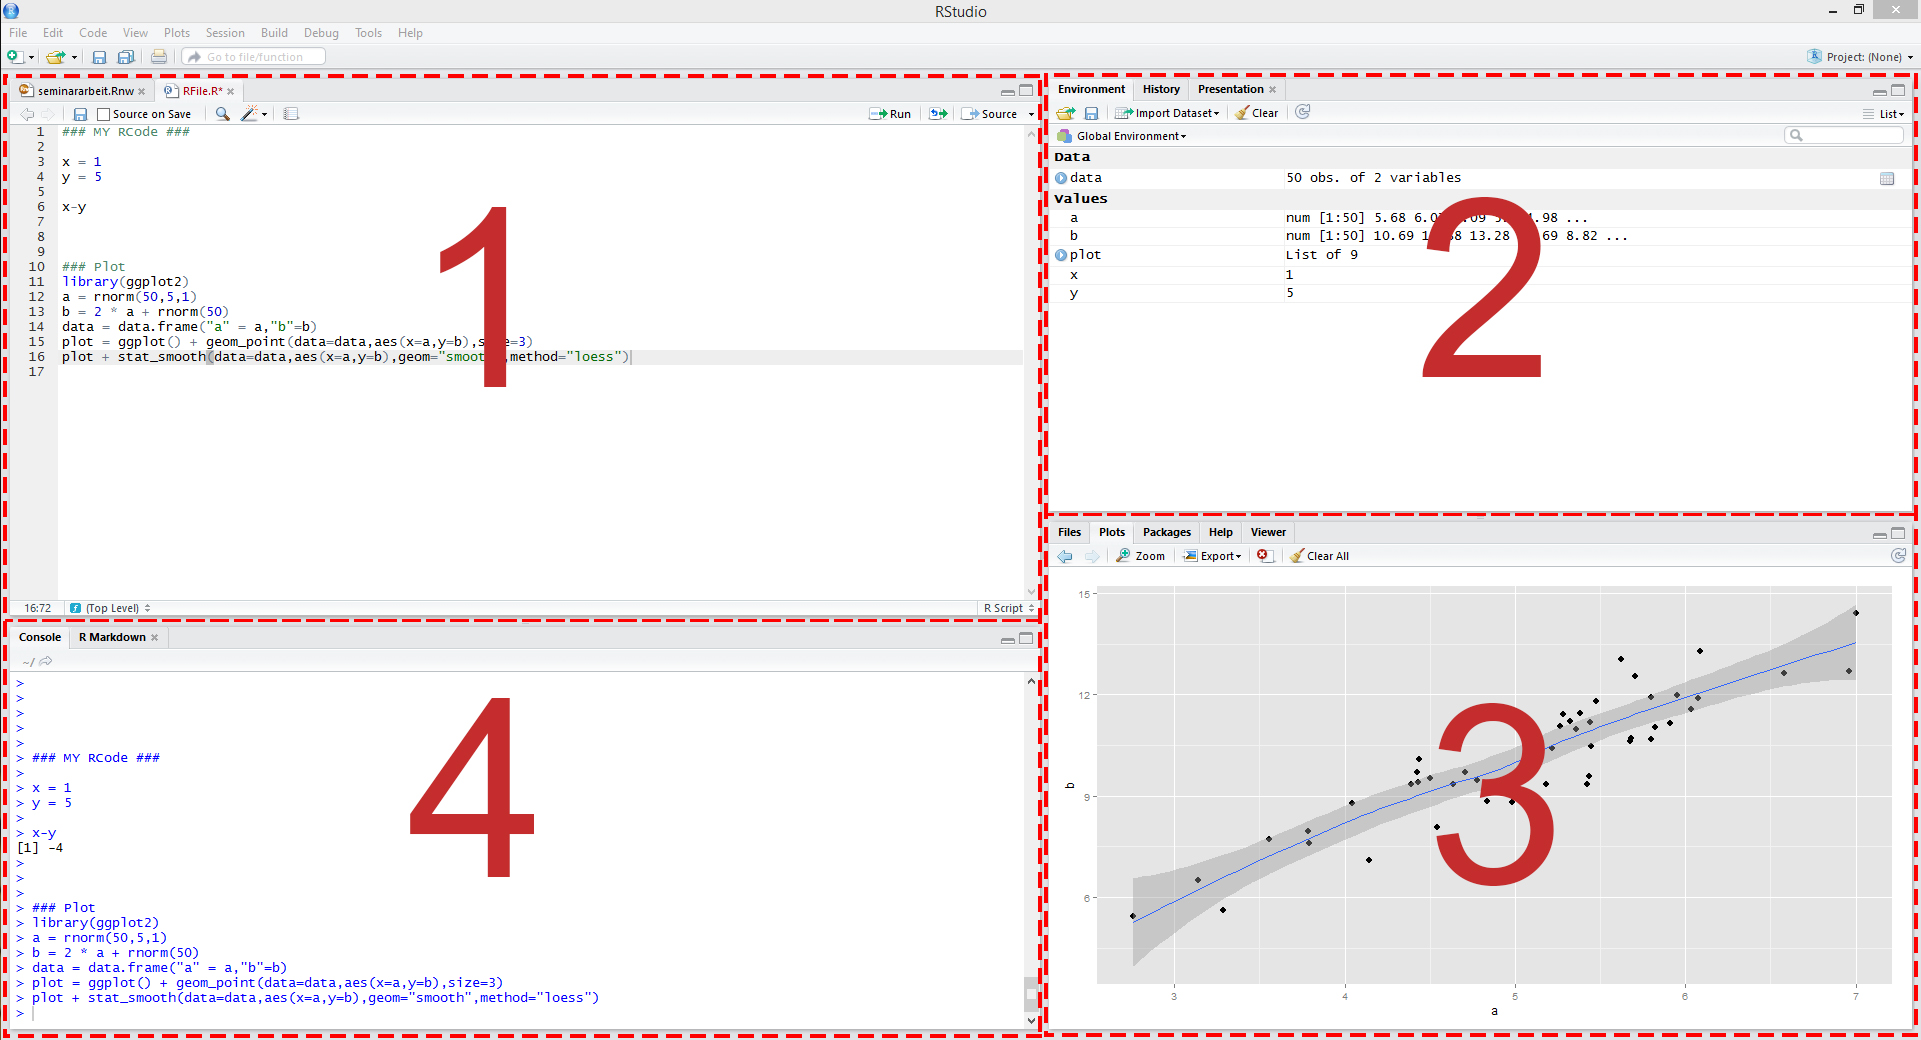
\includegraphics[width=1\linewidth]{images/rstudio} 

}

\caption{RStudio: the four panes}\label{fig:unnamed-chunk-7}
\end{figure}

\subsubsection*{\texorpdfstring{\texttt{R}
Basics}{ Basics}}\label{basics}
\addcontentsline{toc}{subsubsection}{\texttt{R} Basics}

As mentioned before, this book is not intended to be an introduction to
\texttt{R} but as a guide on how to use its capabilities for
applications commonly encountered in undergraduate econometrics. Those
having basic knowledge in \texttt{R} programming will feel comfortable
starting with Chapter \ref{pt}. This section, however, is meant for
those who have not worked with \texttt{R} or \emph{RStudio} before. If
you at least know how to create objects and call functions, you can skip
it. If you would like to refresh your memories or get a feeling for how
to work with \emph{RStudio}, keep reading.

First of all start \emph{RStudio} and create a new \texttt{R} script by
selecting \emph{File}, \emph{New File}, \emph{R Script}. In the editor
pane, type

\begin{Shaded}
\begin{Highlighting}[]
\DecValTok{1} \OperatorTok{+}\StringTok{ }\DecValTok{1}
\end{Highlighting}
\end{Shaded}

and click on the button labeled \emph{Run} in the top right corner of
the editor. By doing so, your line of code is send to the console and
the result of this operation should be displayed right underneath it. As
you can see, \texttt{R} works just like a calculator. You can do all the
arithmetic calculations by using the corresponding operator (\texttt{+},
\texttt{-}, \texttt{*}, \texttt{/} or \texttt{\textasciicircum{}}). If
you are not sure what the last operator does, try it out and check the
results.

\subsubsection*{Vectors}\label{vectors}
\addcontentsline{toc}{subsubsection}{Vectors}

\texttt{R} is of course more sophisticated than that. We can work with
variables or more generally objects. Objects are defined by using the
assignment operator \texttt{<-}. To create a variable named \texttt{x}
which contains the value \texttt{10} type \texttt{x\ \textless{}-\ 10}
and click the button \emph{Run} yet again. The new variable should have
appeared in the environment pane on the top right. The console however
did not show any results, because our line of code did not contain any
call that creates output. When you now type \texttt{x} in the console
and hit return, you ask \texttt{R} to show you the value of \texttt{x}
and the corresponding value should be printed in the console.

\texttt{x} is a scalar, a vector of length \(1\). You can easily create
longer vectors by using the function \texttt{c()} (\emph{c} for
``concatenate'' or ``combine''). To create a vector \texttt{y}
containing the numbers \(1\) to \(5\) and print it, do the following.

\begin{Shaded}
\begin{Highlighting}[]
\NormalTok{y <-}\StringTok{ }\KeywordTok{c}\NormalTok{(}\DecValTok{1}\NormalTok{, }\DecValTok{2}\NormalTok{, }\DecValTok{3}\NormalTok{, }\DecValTok{4}\NormalTok{, }\DecValTok{5}\NormalTok{)}
\NormalTok{y}
\end{Highlighting}
\end{Shaded}

\begin{verbatim}
## [1] 1 2 3 4 5
\end{verbatim}

You can also create a vector of letters or words. For now just remember
that characters have to be surrounded by quotes, else wise they will be
parsed as object names.

\begin{Shaded}
\begin{Highlighting}[]
\NormalTok{hello <-}\StringTok{ }\KeywordTok{c}\NormalTok{(}\StringTok{"Hello"}\NormalTok{, }\StringTok{"World"}\NormalTok{)}
\end{Highlighting}
\end{Shaded}

Here we have created a vector of length 2 containing the words
\texttt{Hello} and \texttt{World}.

Do not forget to save your script! To do so, select \emph{File},
\emph{Save}.

\subsubsection*{Functions}\label{functions}
\addcontentsline{toc}{subsubsection}{Functions}

You have seen the function \texttt{c()} that can be used to combine
objects. In general, function calls look all the same, a function name
is always followed by round parentheses. Sometimes, the parentheses
include arguments

Here are two simple examples.

\begin{Shaded}
\begin{Highlighting}[]
\NormalTok{z <-}\StringTok{ }\KeywordTok{seq}\NormalTok{(}\DataTypeTok{from =} \DecValTok{1}\NormalTok{, }\DataTypeTok{to =} \DecValTok{5}\NormalTok{, }\DataTypeTok{by =} \DecValTok{1}\NormalTok{)}

\KeywordTok{mean}\NormalTok{(}\DataTypeTok{x =}\NormalTok{ z)}
\end{Highlighting}
\end{Shaded}

\begin{verbatim}
## [1] 3
\end{verbatim}

In the first line we use a function called \texttt{seq()} to create the
exact same vector as we did in the previous section but naming it
\texttt{z}. The function takes on the arguments \texttt{from},
\texttt{to} and \texttt{by} which should be self-explaining. The
function \texttt{mean()} computes the arithmetic mean of its argument
\texttt{x}. Since we pass the vector \texttt{z} as the argument
\texttt{x}, the result is \texttt{3}!

If you are not sure which arguments a function expects, you may consult
the function's documentation. Let's say we are not sure how the
arguments required for \texttt{seq()} work. Then we may type
\texttt{?seq} in the console and by hitting return the documentation
page for that function pops up in the lower right pane of
\emph{RStudio}. In there, the section \emph{Arguments} holds the
information we seek.

On the bottom of almost every help page you find examples on how to use
the corresponding functions. This is very helpful for beginners and we
recommend to look out for those.

\chapter{Hypothesis Tests and Confidence Intervals in Multiple
Regression}\label{htaciimr}

This chapter discusses methods that allow to quantify the sampling
uncertainty in the OLS estimator of the coefficients in multiple
regression models. The basis for this are hypothesis tests and
confidence intervals which, just as for the simple linear regression
model, can be computed using basic \texttt{R} functions. We will also
tackle the issue of testing joint hypotheses on these coefficients.

Make sure the packages \texttt{AER} \citep{R-AER} and \texttt{stargazer}
\citep{R-stargazer} are installed before you go ahead and replicate the
examples. The safest way to do so is by checking whether the following
code chunk executes without any issues.

\begin{Shaded}
\begin{Highlighting}[]
\KeywordTok{library}\NormalTok{(AER)}
\KeywordTok{library}\NormalTok{(stargazer)}
\end{Highlighting}
\end{Shaded}

\section{Hypothesis Tests and Confidence Intervals for a Single
Coefficient}\label{hypothesis-tests-and-confidence-intervals-for-a-single-coefficient}

We first discuss how to compute standard errors, how to test hypotheses
and how to construct confidence intervals for a single regression
coefficient \(\beta_j\) in a multiple regression model. The basic idea
is summarized in Key Concept 7.1.

\begin{keyconcepts}[Testing the Hypothesis $\beta_j = \beta_{j,0}$
                    Against the Alternative $\beta_j \neq \beta_{j,0}$]{7.1}
\begin{enumerate}
\item Compute the standard error of $\hat{\beta_j}$
\item Compute the $t$-statistic,
$$t^{act} = \frac{\hat{\beta}_j - \beta_{j,0}} {SE(\hat{\beta_j})}$$
\item Compute the $p$-value,
$$p\text{-value} = 2 \Phi(-|t^{act}|)$$
where $t^{act}$ is the value of the $t$-statistic actually computed. Reject the hypothesis at the 5\% significance level if the $p$-value is less than $0.05$ or, equivalently, if $|t^{act}| > 1.96$. \end{enumerate}\vspace{0.5cm}

The standard error and (typically) the $t$-statistic and the corresponding $p$-value for testing $\beta_j = 0$ are computed automatically by suitable \texttt{R} functions, e.g., by \texttt{summary()}.
\end{keyconcepts}

Testing a single hypothesis about the significance of a coefficient in
the multiple regression model proceeds as in in the simple regression
model.

You can easily see this by inspecting the coefficient summary of the
regression model

\[ TestScore = \beta_0 + \beta_1 \times size  \beta_2 \times english + u \]

already discussed in Chapter \ref{rmwmr}. Let us review this:

\begin{Shaded}
\begin{Highlighting}[]
\NormalTok{model <-}\StringTok{ }\KeywordTok{lm}\NormalTok{(score }\OperatorTok{~}\StringTok{ }\NormalTok{size }\OperatorTok{+}\StringTok{ }\NormalTok{english, }\DataTypeTok{data =}\NormalTok{ CASchools)}
\KeywordTok{coeftest}\NormalTok{(model, }\DataTypeTok{vcov. =} \KeywordTok{vcovHC}\NormalTok{(model, }\DataTypeTok{type =} \StringTok{"HC1"}\NormalTok{))}
\end{Highlighting}
\end{Shaded}

\begin{verbatim}
## 
## t test of coefficients:
## 
##               Estimate Std. Error  t value Pr(>|t|)    
## (Intercept) 686.032245   8.728225  78.5993  < 2e-16 ***
## size         -1.101296   0.432847  -2.5443  0.01131 *  
## english      -0.649777   0.031032 -20.9391  < 2e-16 ***
## ---
## Signif. codes:  0 '***' 0.001 '**' 0.01 '*' 0.05 '.' 0.1 ' ' 1
\end{verbatim}

You may check that these quantities are computed as in the simple
regression model by computing the \(t\)-statistics or \(p\)-values by
hand using the output above and \texttt{R} as a calculator.

For example, using the definition of the \(p\)-value for a two-sided
test as given in Key Concept 7.1, we can confirm the \(p\)-value for a
test of the hypothesis that the coefficient \(\beta_1\), the coefficient
on \texttt{size}, to be approximately zero.

\begin{Shaded}
\begin{Highlighting}[]
\DecValTok{2} \OperatorTok{*}\StringTok{ }\NormalTok{(}\DecValTok{1} \OperatorTok{-}\StringTok{ }\KeywordTok{pt}\NormalTok{(}
            \KeywordTok{abs}\NormalTok{(}
              \KeywordTok{coeftest}\NormalTok{(model, }\DataTypeTok{vcov. =} \KeywordTok{vcovHC}\NormalTok{(model, }\DataTypeTok{type =} \StringTok{"HC1"}\NormalTok{))[}\DecValTok{2}\NormalTok{, }\DecValTok{3}\NormalTok{]),}
            \DataTypeTok{df =}\NormalTok{ model}\OperatorTok{$}\NormalTok{df.residual))}
\end{Highlighting}
\end{Shaded}

\begin{verbatim}
## [1] 0.01130921
\end{verbatim}

\begin{keyconcepts}[Confidence Intervals for a Single Coefficient in Multiple Regression]{7.2}
A $95\%$ two-sided confidence interval for the coefficient $\beta_j$ is an interval that contains the true value of $\beta_j$ with a $95 \%$ probability; that is, it contains the true value of $\beta_j$ in $95 \%$ of repeated samples. Equivalently, it is the set of values of $\beta_j$ that cannot be rejected by a $5 \%$ two-sided hypothesis test. When the sample size is large, the $95 \%$ confidence interval for $\beta_j$ is
$$\left[\hat{\beta_j}- 1.96 \times SE(\hat{\beta}_j), \hat{\beta_j} + 1.96 \times SE(\hat{\beta_j})\right].$$
\end{keyconcepts}

\section{An Application to Test Scores and the Student-Teacher
Ratio}\label{an-application-to-test-scores-and-the-student-teacher-ratio}

Let us take a look at the regression from Section \ref{mofimr} again.

Computing confidence intervals for individual coefficients in the
multiple regression model proceeds as in the simple regression model
using the function \texttt{confint()}.

\begin{Shaded}
\begin{Highlighting}[]
\NormalTok{model <-}\StringTok{ }\KeywordTok{lm}\NormalTok{(score }\OperatorTok{~}\StringTok{ }\NormalTok{size }\OperatorTok{+}\StringTok{ }\NormalTok{english, }\DataTypeTok{data =}\NormalTok{ CASchools)}
\KeywordTok{confint}\NormalTok{(model)}
\end{Highlighting}
\end{Shaded}

\begin{verbatim}
##                   2.5 %      97.5 %
## (Intercept) 671.4640580 700.6004311
## size         -1.8487969  -0.3537944
## english      -0.7271113  -0.5724424
\end{verbatim}

To obtain confidence intervals at another level, say \(90\%\), just set
the argument \texttt{level} in our call of \texttt{confint()}
accordingly.

\begin{Shaded}
\begin{Highlighting}[]
\KeywordTok{confint}\NormalTok{(model, }\DataTypeTok{level =} \FloatTok{0.9}\NormalTok{)}
\end{Highlighting}
\end{Shaded}

\begin{verbatim}
##                     5 %        95 %
## (Intercept) 673.8145793 698.2499098
## size         -1.7281904  -0.4744009
## english      -0.7146336  -0.5849200
\end{verbatim}

The output now reports the desired \(90\%\) confidence intervals for all
coefficients.

A disadvantage of \texttt{confint()} is that is does not use robust
standard errors to compute the confidence interval. For large-sample
confidence intervals, this is quickly done manually as follows.

\begin{Shaded}
\begin{Highlighting}[]
\CommentTok{# compute robust standard errors}
\NormalTok{rob_se <-}\StringTok{ }\KeywordTok{diag}\NormalTok{(}\KeywordTok{vcovHC}\NormalTok{(model, }\DataTypeTok{type =} \StringTok{"HC1"}\NormalTok{))}\OperatorTok{^}\FloatTok{0.5}

\CommentTok{# compute robust 95% confidence intervals}
\KeywordTok{rbind}\NormalTok{(}
  \StringTok{"lower"}\NormalTok{ =}\StringTok{ }\KeywordTok{coef}\NormalTok{(model) }\OperatorTok{-}\StringTok{ }\KeywordTok{qnorm}\NormalTok{(}\FloatTok{0.975}\NormalTok{) }\OperatorTok{*}\StringTok{ }\NormalTok{rob_se,}
  \StringTok{"upper"}\NormalTok{ =}\StringTok{ }\KeywordTok{coef}\NormalTok{(model) }\OperatorTok{+}\StringTok{ }\KeywordTok{qnorm}\NormalTok{(}\FloatTok{0.975}\NormalTok{) }\OperatorTok{*}\StringTok{ }\NormalTok{rob_se}
\NormalTok{)}
\end{Highlighting}
\end{Shaded}

\begin{verbatim}
##       (Intercept)       size    english
## lower    668.9252 -1.9496606 -0.7105980
## upper    703.1393 -0.2529307 -0.5889557
\end{verbatim}

\begin{Shaded}
\begin{Highlighting}[]
\CommentTok{# compute robust 90% confidence intervals}

\KeywordTok{rbind}\NormalTok{(}
  \StringTok{"lower"}\NormalTok{ =}\StringTok{ }\KeywordTok{coef}\NormalTok{(model) }\OperatorTok{-}\StringTok{ }\KeywordTok{qnorm}\NormalTok{(}\FloatTok{0.95}\NormalTok{) }\OperatorTok{*}\StringTok{ }\NormalTok{rob_se,}
  \StringTok{"upper"}\NormalTok{ =}\StringTok{ }\KeywordTok{coef}\NormalTok{(model) }\OperatorTok{+}\StringTok{ }\KeywordTok{qnorm}\NormalTok{(}\FloatTok{0.95}\NormalTok{) }\OperatorTok{*}\StringTok{ }\NormalTok{rob_se}
\NormalTok{)}
\end{Highlighting}
\end{Shaded}

\begin{verbatim}
##       (Intercept)       size    english
## lower    671.6756 -1.8132659 -0.7008195
## upper    700.3889 -0.3893254 -0.5987341
\end{verbatim}

Knowing how to use \texttt{R} to make inference about the coefficients
in multiple regression models, you can now answer the following
question:

Can the null hypothesis that a change in the student-teacher ratio,
\texttt{size}, has no significant influence on test scores,
\texttt{scores}, --- if we control for the percentage of students
learning English in the district, \texttt{english}, --- be rejected at
the \(10\%\) and the \(5\%\) level of significance?

The output above shows that zero is not an element of the confidence
interval for the coefficient on \texttt{size} such that we can reject
the null hypothesis at significance levels of \(5\%\) and \(10\%\). The
same conclusion can be made via the \(p\)-value for \texttt{size}:
\(0.00398 < 0.05 = \alpha\).

Note that rejection at the \(5\%\)-level implies rejection at the
\(10\%\) level (why?).

Recall from Chapter \ref{cifrc} the \(95\%\) confidence interval
computed above \emph{does not} tell us that a one-unit decrease in the
student-teacher ratio has an effect on test scores that lies in the
interval with a lower bound of \(-1.9497\) and an upper bound of
\(-0.2529\). Once a confidence interval has been computed, a
probabilistic statement like this is wrong: either the interval contains
the true parameter or it does not. We do not know which is true.

\subsection*{Another Augmentation of the
Model}\label{another-augmentation-of-the-model}
\addcontentsline{toc}{subsection}{Another Augmentation of the Model}

What is the average effect on test scores of reducing the
student-teacher ratio when the expenditures per pupil and the percentage
of english learning pupils are held constant?

Let us augment our model by an additional regressor that is a measure
for expenditure per pupil. Using \texttt{?CASchools} we find that
\texttt{CASchools} contains the variable \texttt{expenditure}, which
provides expenditure per student.

Our model now is
\[ TestScore = \beta_0 + \beta_1 \times size + \beta_2 \times english + \beta_3 \times expenditure + u \]

with \(expenditure\) the total amount of expenditure per pupil in the
district (thousands of dollars).

Let us now estimate the model:

\begin{Shaded}
\begin{Highlighting}[]
\CommentTok{# scale expenditure to thousands of dollars}
\NormalTok{CASchools}\OperatorTok{$}\NormalTok{expenditure <-}\StringTok{ }\NormalTok{CASchools}\OperatorTok{$}\NormalTok{expenditure}\OperatorTok{/}\DecValTok{1000}

\CommentTok{# estimate the model}
\NormalTok{model <-}\StringTok{ }\KeywordTok{lm}\NormalTok{(score }\OperatorTok{~}\StringTok{ }\NormalTok{size }\OperatorTok{+}\StringTok{ }\NormalTok{english }\OperatorTok{+}\StringTok{ }\NormalTok{expenditure, }\DataTypeTok{data =}\NormalTok{ CASchools)}
\KeywordTok{coeftest}\NormalTok{(model, }\DataTypeTok{vcov. =} \KeywordTok{vcovHC}\NormalTok{(model, }\DataTypeTok{type =} \StringTok{"HC1"}\NormalTok{))}
\end{Highlighting}
\end{Shaded}

\begin{verbatim}
## 
## t test of coefficients:
## 
##               Estimate Std. Error  t value Pr(>|t|)    
## (Intercept) 649.577947  15.458344  42.0212  < 2e-16 ***
## size         -0.286399   0.482073  -0.5941  0.55277    
## english      -0.656023   0.031784 -20.6398  < 2e-16 ***
## expenditure   3.867901   1.580722   2.4469  0.01482 *  
## ---
## Signif. codes:  0 '***' 0.001 '**' 0.01 '*' 0.05 '.' 0.1 ' ' 1
\end{verbatim}

The estimated effect of a one unit change in the student-teacher ratio
on test scores with expenditure and the share of english learning pupils
held constant is \(-0.29\), which is rather small. What is more, the
coefficient on \(size\) is not significantly different from zero anymore
even at \(10\%\) since \(p\text{-value}=0.55\). Can you come up with an
interpretation for these findings (see Chapter 7.1 of the book)? The
insignificance of \(\hat\beta_1\) could be due to a larger standard
error of \(\hat{\beta}_1\) resulting from adding \(expenditure\) to the
model so that we estimate the coefficient on \(size\) less precisely.
This illustrates the issue of strongly correlated regressors (imperfect
multicollinearity). The correlation between \(size\) and \(expenditure\)
can be computed using \texttt{cor()}.

\begin{Shaded}
\begin{Highlighting}[]
\CommentTok{# compute the sample correlation between 'size' and 'expenditure'}
\KeywordTok{cor}\NormalTok{(CASchools}\OperatorTok{$}\NormalTok{size, CASchools}\OperatorTok{$}\NormalTok{expenditure)}
\end{Highlighting}
\end{Shaded}

\begin{verbatim}
## [1] -0.6199822
\end{verbatim}

Altogether, we conclude that the new model provides no evidence that
changing the student-teacher ratio, e.g., by hiring new teachers, has
any effect on the test scores while keeping expenditures per student and
the share of English learners constant.

\section{Joint Hypothesis Testing Using the
F-Statistic}\label{joint-hypothesis-testing-using-the-f-statistic}

The estimated model is

\[ \widehat{TestScore} = \underset{(15.21)}{649.58} -\underset{(0.48)}{0.29} \times size - \underset{(0.04)}{0.66} \times english + \underset{(1.41)}{3.87} \times expenditure. \]

Now, can we reject the hypothesis that the coefficient on \(size\)
\emph{and} the coefficient on \(expenditure\) are zero? To answer this,
we have to resort to joint hypothesis tests. A joint hypothesis imposes
restrictions on multiple regression coefficients. This is different from
conducting individual \(t\)-tests where a restriction is imposed on a
single coefficient. Chapter 7.2 of the book explains why testing
hypotheses about the model coefficients one at a time is different from
testing them jointly.

The homoskedasticity-only \(F\)-Statistic is given by

\[ F = \frac{(SSR_{restricted} - SSR_{unrestricted})/q}{SSR_{unrestricted} / (n-k-1)} \]

with \(SSR_{restricted}\) being the sum of squared residuals from the
restricted regression, i.e., the regression where we impose the
restriction. \(SSR_{unrestricted}\) is the sum of squared residuals from
the full model, \(q\) is the number of restrictions under the null and
\(k\) is the number of regressors in the unrestricted regression.

It is fairly easy to conduct \(F\)-tests in \texttt{R}. We can use the
function \texttt{linearHypothesis()}contained in the package
\texttt{car}.

\begin{Shaded}
\begin{Highlighting}[]
\CommentTok{# estimate the multiple regression model}
\NormalTok{model <-}\StringTok{ }\KeywordTok{lm}\NormalTok{(score }\OperatorTok{~}\StringTok{ }\NormalTok{size }\OperatorTok{+}\StringTok{ }\NormalTok{english }\OperatorTok{+}\StringTok{ }\NormalTok{expenditure, }\DataTypeTok{data =}\NormalTok{ CASchools)}

\CommentTok{# execute the function on the model object and provide both linear restrictions }
\CommentTok{# to be tested as strings}
\KeywordTok{linearHypothesis}\NormalTok{(model, }\KeywordTok{c}\NormalTok{(}\StringTok{"size=0"}\NormalTok{, }\StringTok{"expenditure=0"}\NormalTok{))}
\end{Highlighting}
\end{Shaded}

\begin{verbatim}
## Linear hypothesis test
## 
## Hypothesis:
## size = 0
## expenditure = 0
## 
## Model 1: restricted model
## Model 2: score ~ size + english + expenditure
## 
##   Res.Df   RSS Df Sum of Sq      F   Pr(>F)    
## 1    418 89000                                 
## 2    416 85700  2    3300.3 8.0101 0.000386 ***
## ---
## Signif. codes:  0 '***' 0.001 '**' 0.01 '*' 0.05 '.' 0.1 ' ' 1
\end{verbatim}

The output reveals that the \(F\)-statistic for this joint hypothesis
test is about \(8.01\) and the corresponding \(p\)-value is \(0.0004\).
Thus, we can reject the null hypothesis that both coefficients are zero
at any level of significance commonly used in practice.

A heteroskedasticity-robust version of this \(F\)-test (which leads to
the same conclusion) can be conducted as follows.

\begin{Shaded}
\begin{Highlighting}[]
\CommentTok{# heteroskedasticity-robust F-test}
\KeywordTok{linearHypothesis}\NormalTok{(model, }\KeywordTok{c}\NormalTok{(}\StringTok{"size=0"}\NormalTok{, }\StringTok{"expenditure=0"}\NormalTok{), }\DataTypeTok{white.adjust =} \StringTok{"hc1"}\NormalTok{)}
\end{Highlighting}
\end{Shaded}

\begin{verbatim}
## Linear hypothesis test
## 
## Hypothesis:
## size = 0
## expenditure = 0
## 
## Model 1: restricted model
## Model 2: score ~ size + english + expenditure
## 
## Note: Coefficient covariance matrix supplied.
## 
##   Res.Df Df      F   Pr(>F)   
## 1    418                      
## 2    416  2 5.4337 0.004682 **
## ---
## Signif. codes:  0 '***' 0.001 '**' 0.01 '*' 0.05 '.' 0.1 ' ' 1
\end{verbatim}

The standard output of a model summary also reports an \(F\)-statistic
and the corresponding \(p\)-value. The null hypothesis belonging to this
\(F\)-test is that \emph{all} of the population coefficients in the
model except for the intercept are zero, so the hypotheses are
\[H_0: \beta_1=0, \ \beta_2 =0, \ \beta_3 =0 \quad \text{vs.} \quad H_1: \beta_j \neq 0 \ \text{for at least one} \ j=1,2,3.\]

This is also called the \emph{overall regression \(F\)-statistic} and
the null hypothesis is obviously different from testing if only
\(\beta_1\) and \(\beta_3\) are zero.

We now check whether the \(F\)-statistic belonging to the \(p\)-value
listed in the model's summary coincides with the result reported by
\texttt{linearHypothesis()}.

\begin{Shaded}
\begin{Highlighting}[]
\CommentTok{# execute the function on the model object and provide the restrictions }
\CommentTok{# to be tested as a character vector}
\KeywordTok{linearHypothesis}\NormalTok{(model, }\KeywordTok{c}\NormalTok{(}\StringTok{"size=0"}\NormalTok{, }\StringTok{"english=0"}\NormalTok{, }\StringTok{"expenditure=0"}\NormalTok{))}
\end{Highlighting}
\end{Shaded}

\begin{verbatim}
## Linear hypothesis test
## 
## Hypothesis:
## size = 0
## english = 0
## expenditure = 0
## 
## Model 1: restricted model
## Model 2: score ~ size + english + expenditure
## 
##   Res.Df    RSS Df Sum of Sq      F    Pr(>F)    
## 1    419 152110                                  
## 2    416  85700  3     66410 107.45 < 2.2e-16 ***
## ---
## Signif. codes:  0 '***' 0.001 '**' 0.01 '*' 0.05 '.' 0.1 ' ' 1
\end{verbatim}

\begin{Shaded}
\begin{Highlighting}[]
\CommentTok{# Access the overall F-statistic from the model's summary}
\KeywordTok{summary}\NormalTok{(model)}\OperatorTok{$}\NormalTok{fstatistic}
\end{Highlighting}
\end{Shaded}

\begin{verbatim}
##    value    numdf    dendf 
## 107.4547   3.0000 416.0000
\end{verbatim}

The entry \texttt{value} is the overall \(F\)-statistics and it equals
the result of \texttt{linearHypothesis()}. The \(F\)-test rejects the
null hypothesis that the model has no power in explaining test scores.
It is important to know that the \(F\)-statistic reported by
\texttt{summary} is \emph{not} robust to heteroskedasticity!

\section{Confidence Sets for Multiple
Coefficients}\label{confidence-sets-for-multiple-coefficients}

Based on the \(F\)-statistic that we have previously encountered, we can
specify confidence sets. Confidence sets are analogous to confidence
intervals for single coefficients. As such, confidence sets consist of
\emph{combinations} of coefficients that contain the true combination of
coefficients in, say, \(95\%\) of all cases if we could repeatedly draw
random samples, just like in the univariate case. Put differently, a
confidence set is the set of all coefficient combinations for which we
cannot reject the corresponding joint null hypothesis tested using an
\(F\)-test.

The confidence set for two coefficients an ellipse which is centered
around the point defined by both coefficient estimates. Again, there is
a very convenient way to plot the confidence set for two coefficients of
model objects, namely the function \texttt{confidenceEllipse()} from the
\texttt{car} package.

We now plot the \(95\%\) confidence ellipse for the coefficients on
\texttt{size} and \texttt{expenditure} from the regression conducted
above. By specifying the additional argument \texttt{fill}, the
confidence set is colored.

\begin{Shaded}
\begin{Highlighting}[]
\CommentTok{# Draw the 95% confidence set for coefficients on size and expenditure}
\KeywordTok{confidenceEllipse}\NormalTok{(model, }
                  \DataTypeTok{fill =}\NormalTok{ T, }
                  \DataTypeTok{which.coef =} \KeywordTok{c}\NormalTok{(}\StringTok{"size"}\NormalTok{, }\StringTok{"expenditure"}\NormalTok{),}
                  \DataTypeTok{main =} \StringTok{"95% Confidence Set"}\NormalTok{)}
\end{Highlighting}
\end{Shaded}

\begin{center}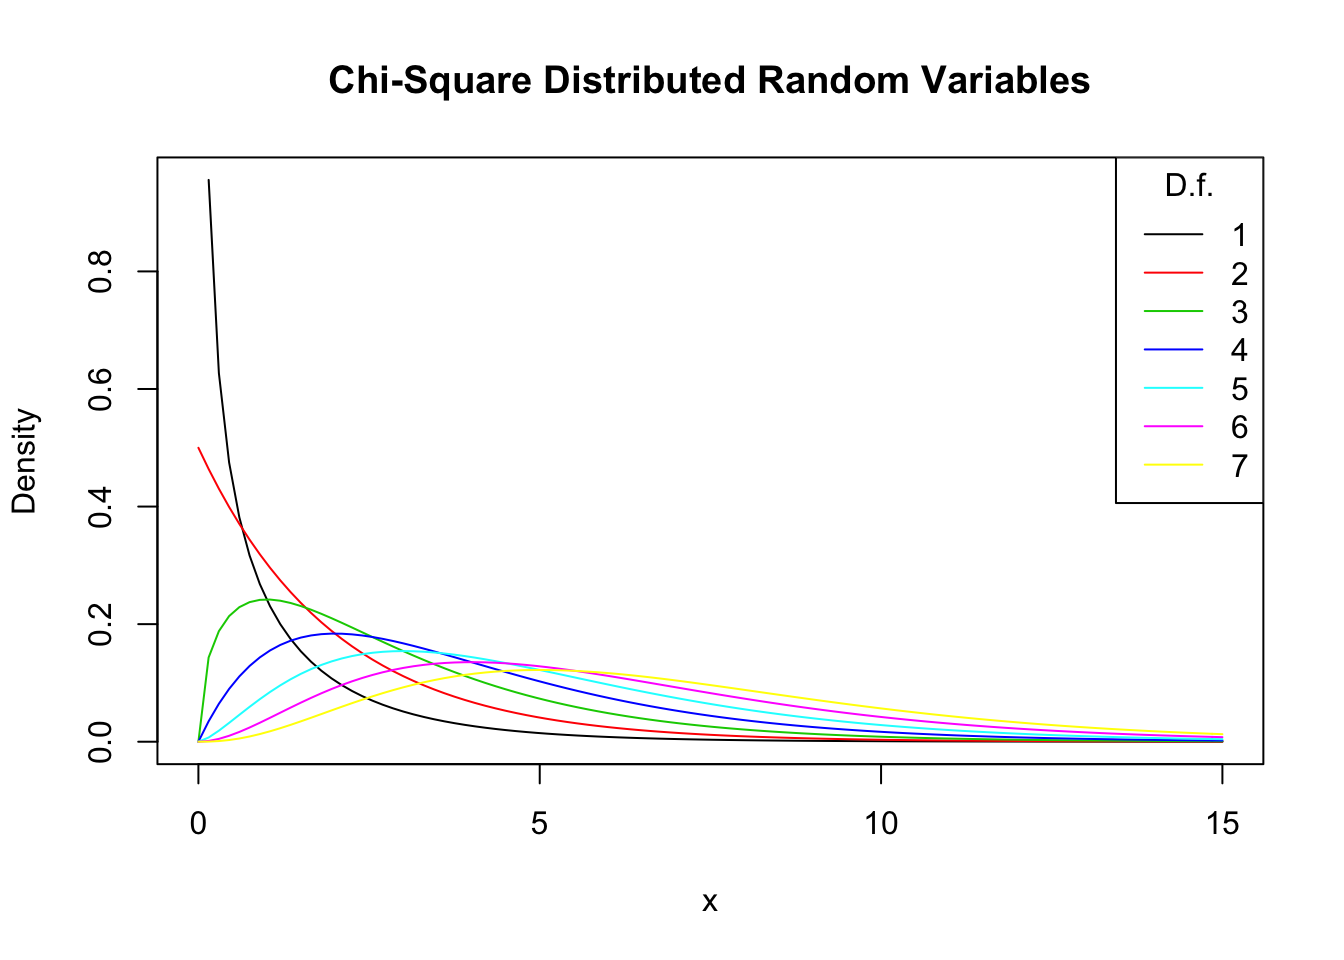
\includegraphics{URFITE_files/figure-latex/unnamed-chunk-27-1} \end{center}

We see that the ellipse is centered around \((-0.29, 3.87)\), the pair
of coefficients estimates on \(size\) and \(expenditure\). What is more,
\((0,0)\) is not element of the \(95\%\) confidence set so that we can
reject \(H_0: \beta_1 = 0, \ \beta_3 = 0\).

By default, \texttt{confidenceEllipse()} uses homoskedasticity-only
standard errors. The following code chunk shows how compute a robust
confidence ellipse and how to overlay it with the previous plot.

\begin{Shaded}
\begin{Highlighting}[]
\CommentTok{# Draw the 95% confidence set for coefficients on size and expenditure (robust)}
\KeywordTok{confidenceEllipse}\NormalTok{(model, }
                  \DataTypeTok{fill =}\NormalTok{ T,}
                  \DataTypeTok{lwd =} \DecValTok{0}\NormalTok{,}
                  \DataTypeTok{which.coef =} \KeywordTok{c}\NormalTok{(}\StringTok{"size"}\NormalTok{, }\StringTok{"expenditure"}\NormalTok{),}
                  \DataTypeTok{main =} \StringTok{"95% Confidence Sets"}\NormalTok{,}
                  \DataTypeTok{vcov. =} \KeywordTok{vcovHC}\NormalTok{(model, }\DataTypeTok{type =} \StringTok{"HC1"}\NormalTok{),}
                  \DataTypeTok{col =} \StringTok{"red"}\NormalTok{)}
                  
\CommentTok{# Draw the 95% confidence set for coefficients on size and expenditure}
\KeywordTok{confidenceEllipse}\NormalTok{(model, }
                  \DataTypeTok{fill =}\NormalTok{ T,}
                  \DataTypeTok{lwd =} \DecValTok{0}\NormalTok{,}
                  \DataTypeTok{which.coef =} \KeywordTok{c}\NormalTok{(}\StringTok{"size"}\NormalTok{, }\StringTok{"expenditure"}\NormalTok{),}
                  \DataTypeTok{add =}\NormalTok{ T)}
\end{Highlighting}
\end{Shaded}

\begin{center}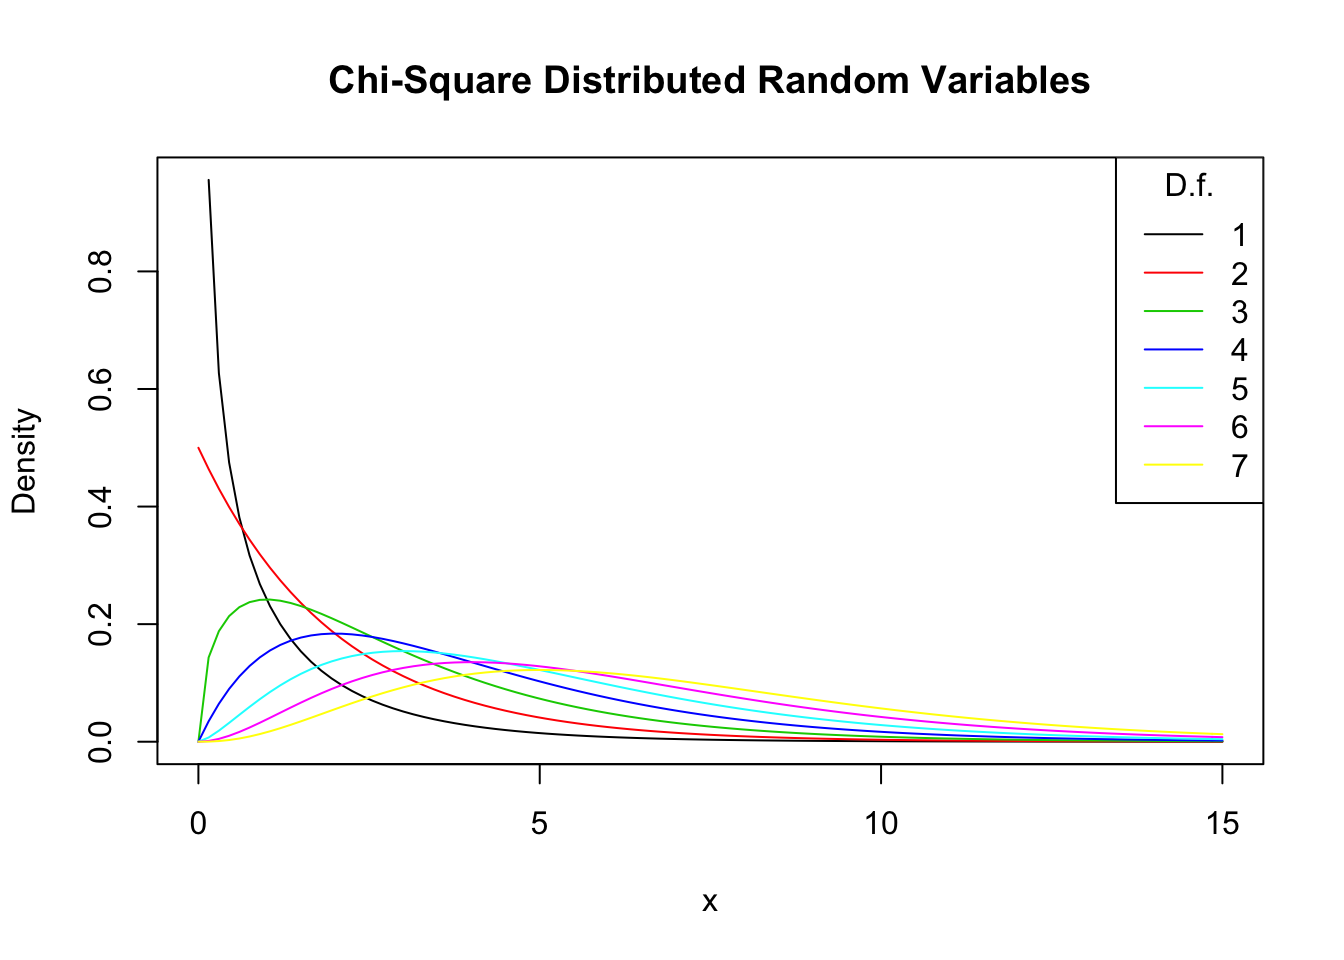
\includegraphics{URFITE_files/figure-latex/unnamed-chunk-28-1} \end{center}

As the robust standard errors are slightly larger than those valid under
homoskedasticity only in this case, the robust confidence set is
slightly larger. This is analogous to the confidence intervals for the
individual coefficients.

\section{Model Specification for Multiple
Regression}\label{model-specification-for-multiple-regression}

Choosing a regression specification, i.e.~selecting, the variables to be
included in a regression model, is a difficult task. However, there are
some guidelines on how to proceed. The goal is clear: obtaining an
unbiased and precise estimate of the causal effect of interest. As a
starting point, think about omitted variables, that is, to avoid
possible bias by using suitable control variables. Omitted variables
bias in the context of multiple regression is explained in Key Concept
7.3. A second step could be to compare different specifications by
measures of fit. However, as we shall see one should not rely solely on
\(\overline{R^2}\).

\begin{keyconcepts}[Omitted Variable Bias in Multiple Regression]{7.3}
Omitted variable bias is the bias in the OLS estimator that arises when regressors correlate with an omitted variable. For omitted variable bias to arise, two things must be true:\newline

\begin{enumerate}
\item At least one of the included regressors must be correlated with the omitted variable. 
\item The omitted variable must be a determinant of the dependent variable, $Y$.
\end{enumerate}

\end{keyconcepts}

We now discuss an example were we face a potential omitted variable bias
in a multiple regression model:

Consider again the estimated regression equation

\[ \widehat{TestScore} = \underset{(8.7)}{686.0} - \underset{(0.43)}{1.10} \times size - \underset{(0.031)}{0.650} \times english. \]

We are interested in estimating the causal effect of class size on test
score. There might be a bias due to omitting ``outside learning
opportunities'' from our regression since such a measure could be a
determinant of the students' test scores and could also be correlated
with both regressors already included in the model (so that both
conditions of Key Concept 7.3 are fulfilled). ``Outside learning
opportunities'' are a complicated concept that is difficult to quantify.
A surrogate we can consider instead is the students' economic background
which likely are strongly related to outside learning opportunities:
think of wealthy parents that are able to provide time and/or money for
private tuition of their children. We thus augment the model with the
variable \texttt{lunch}, the percentage of students that qualify for a
free or subsidized lunch in school due to family incomes below a certain
threshold, and reestimate the model.

\begin{Shaded}
\begin{Highlighting}[]
\CommentTok{# estimate the model and print the summary to console}
\NormalTok{model <-}\StringTok{ }\KeywordTok{lm}\NormalTok{(score }\OperatorTok{~}\StringTok{ }\NormalTok{size }\OperatorTok{+}\StringTok{ }\NormalTok{english }\OperatorTok{+}\StringTok{ }\NormalTok{lunch, }\DataTypeTok{data =}\NormalTok{ CASchools)}
\KeywordTok{coeftest}\NormalTok{(model, }\DataTypeTok{vcov. =} \KeywordTok{vcovHC}\NormalTok{(model, }\DataTypeTok{type =} \StringTok{"HC1"}\NormalTok{))}
\end{Highlighting}
\end{Shaded}

\begin{verbatim}
## 
## t test of coefficients:
## 
##               Estimate Std. Error  t value  Pr(>|t|)    
## (Intercept) 700.149957   5.568453 125.7351 < 2.2e-16 ***
## size         -0.998309   0.270080  -3.6963 0.0002480 ***
## english      -0.121573   0.032832  -3.7029 0.0002418 ***
## lunch        -0.547345   0.024107 -22.7046 < 2.2e-16 ***
## ---
## Signif. codes:  0 '***' 0.001 '**' 0.01 '*' 0.05 '.' 0.1 ' ' 1
\end{verbatim}

Thus, the estimated regression line is

\[ \widehat{TestScore} = \underset{(5.56)}{700.15} - \underset{(0.27)}{1.00} \times size - \underset{(0.03)}{0.12} \times english - \underset{(0.02)}{0.55} \times lunch. \]

We observe no substantial changes in the conclusion about the effect of
\(size\) on \(TestScore\): the coefficient on \(size\) changes by only
\(0.1\) and retains its significance.

Although the difference in estimated coefficients is not big in this
case, it is useful to keep \texttt{lunch} to make the assumption of
conditional mean independence more credible (see Chapter 7.5 of the
book).

\subsection*{Model Specification in Theory and in
Practice}\label{model-specification-in-theory-and-in-practice}
\addcontentsline{toc}{subsection}{Model Specification in Theory and in
Practice}

Key Concept 7.4 lists some common pitfalls when using \(R^2\) and
\(\overline{R^2}\) to evaluate the predictive ability of regression
models.

\begin{keyconcepts}[$R^2$ and $\overline{R^2}$: What They Tell You --- and What They Do not]{7.4}
The $R^2$ and $\overline{R^2}$ tell you whether the regressors are good at explaining the variation of the independent variable in the sample. If the $R^2$ (or $\overline{R^2}$) is nearly $1$, then the regressors produce a good prediction of the dependent variable in that sample, in the sense that the variance of OLS residuals is small compared to the variance of the dependent variable. If the $R^2$ (or $\overline{R^2}$) is nearly $0$, the opposite is true.\newline

The $R^2$ and $\overline{R^2}$ do \textit{not} tell you whether:\newline

\begin{enumerate}
\item An included variable is statistically significant. 
\item The regressors are the true cause of the movements in the dependent variable.
\item There is omitted variable bias.
\item You have chosen the most appropriate set of regressors.
\end{enumerate}
\end{keyconcepts}

For example, think of regressing \(TestScore\) on \(PLS\) which measures
the available parking lot space in thousand square feet. You are likely
to observe a significant coefficient of reasonable magnitude and
moderate to high values for \(R^2\) and \(\overline{R^2}\). The reason
for this is that parking lot space is correlated with many determinants
of the test score like location, class size, financial endowment and so
on. Although we do not have observations on \(PLS\), we can use
\texttt{R} to generate some relatively realistic data.

\begin{Shaded}
\begin{Highlighting}[]
\CommentTok{# set seed for reproducibility}
\KeywordTok{set.seed}\NormalTok{(}\DecValTok{1}\NormalTok{)}

\CommentTok{# generate observations for parking lot space}
\NormalTok{CASchools}\OperatorTok{$}\NormalTok{PLS <-}\StringTok{ }\KeywordTok{c}\NormalTok{(}\DecValTok{22} \OperatorTok{*}\StringTok{ }\NormalTok{CASchools}\OperatorTok{$}\NormalTok{income }
                   \OperatorTok{-}\StringTok{ }\DecValTok{15} \OperatorTok{*}\StringTok{ }\NormalTok{CASchools}\OperatorTok{$}\NormalTok{size }
                   \OperatorTok{+}\StringTok{ }\FloatTok{0.2} \OperatorTok{*}\StringTok{ }\NormalTok{CASchools}\OperatorTok{$}\NormalTok{expenditure}
                   \OperatorTok{+}\StringTok{ }\KeywordTok{rnorm}\NormalTok{(}\KeywordTok{nrow}\NormalTok{(CASchools), }\DataTypeTok{sd =} \DecValTok{80}\NormalTok{) }\OperatorTok{+}\StringTok{ }\DecValTok{3000}\NormalTok{)}
\end{Highlighting}
\end{Shaded}

\begin{Shaded}
\begin{Highlighting}[]
\CommentTok{# plot parking lot space against test score}
\KeywordTok{plot}\NormalTok{(CASchools}\OperatorTok{$}\NormalTok{PLS, }
\NormalTok{     CASchools}\OperatorTok{$}\NormalTok{score,}
     \DataTypeTok{xlab =} \StringTok{"Parking Lot Space"}\NormalTok{,}
     \DataTypeTok{ylab =} \StringTok{"Test Score"}\NormalTok{,}
     \DataTypeTok{pch =} \DecValTok{20}\NormalTok{,}
     \DataTypeTok{col =} \StringTok{"steelblue"}\NormalTok{)}
\end{Highlighting}
\end{Shaded}

\begin{center}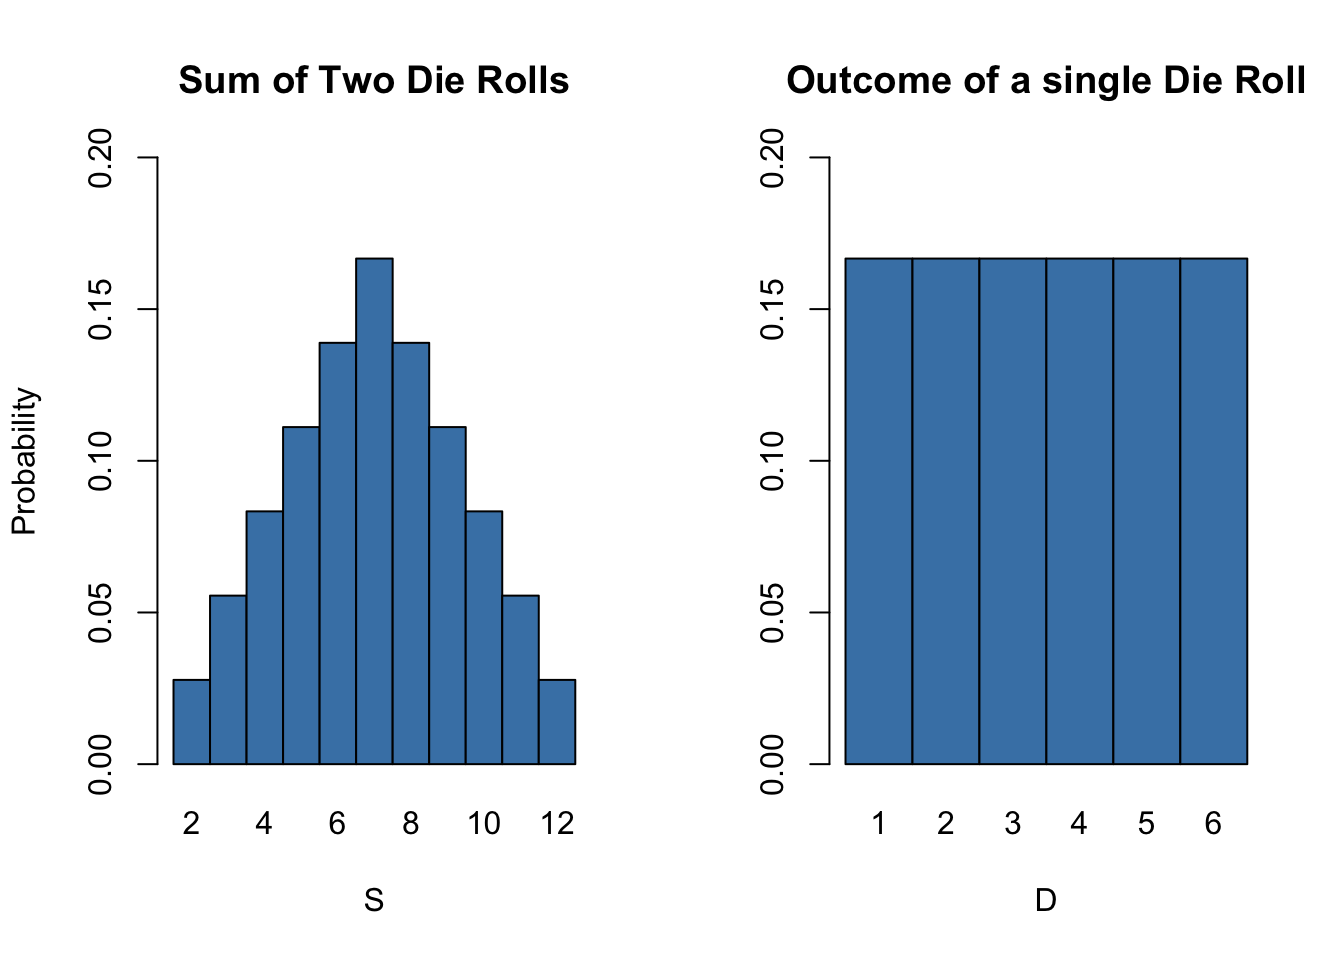
\includegraphics{URFITE_files/figure-latex/unnamed-chunk-35-1} \end{center}

\begin{Shaded}
\begin{Highlighting}[]
\CommentTok{# regress test score on PLS}
\KeywordTok{summary}\NormalTok{(}\KeywordTok{lm}\NormalTok{(score }\OperatorTok{~}\StringTok{ }\NormalTok{PLS, }\DataTypeTok{data =}\NormalTok{ CASchools))}
\end{Highlighting}
\end{Shaded}

\begin{verbatim}
## 
## Call:
## lm(formula = score ~ PLS, data = CASchools)
## 
## Residuals:
##     Min      1Q  Median      3Q     Max 
## -42.608 -11.049   0.342  12.558  37.105 
## 
## Coefficients:
##              Estimate Std. Error t value Pr(>|t|)    
## (Intercept) 4.897e+02  1.227e+01   39.90   <2e-16 ***
## PLS         4.002e-02  2.981e-03   13.43   <2e-16 ***
## ---
## Signif. codes:  0 '***' 0.001 '**' 0.01 '*' 0.05 '.' 0.1 ' ' 1
## 
## Residual standard error: 15.95 on 418 degrees of freedom
## Multiple R-squared:  0.3013, Adjusted R-squared:  0.2996 
## F-statistic: 180.2 on 1 and 418 DF,  p-value: < 2.2e-16
\end{verbatim}

\(PLS\) is generated as a linear function of \(expenditure\),
\(income\), \(size\) and a random disturbance. Therefore the data
suggest that there is some positive relationship between parking lot
space and test score. In fact, when estimating the model

\begin{align}
TestScore = \beta_0 + \beta_1 \times PLS + u \label{eq:plsmod} 
\end{align}

using \texttt{lm()} we find that the coefficient on \(PLS\) is positive
and significantly different from zero. Also \(R^2\) and
\(\overline{R^2}\) are about \(0.3\) which is a lot more than the
roughly \(0.05\) observed when regressing the test scores on the class
sizes only. This suggests that increasing the parking lot space boosts a
school's test scores and that model \eqref{eq:plsmod} does even better in
explaining heterogeneity in the dependent variable than a model with
\(size\) as the only regressor. Keeping in mind how \(PLS\) is
constructed this comes as no surprise. It is evident that the high
\(R^2\) cannot be used to the conclude that the estimated relation
between parking lot space and test scores is causal: the (relatively)
high \(R^2\) is due to correlation between \(PLS\) and other
determinants and/or control variables. Increasing parking lot space is
\emph{not} an appropriate measure to generate more learning success!

\section{Analysis of the Test Score Data
Set}\label{analysis-of-the-test-score-data-set}

Chapter \ref{rmwmr} and some of the previous sections have stressed that
it is important to include control variables in regression models if it
is plausible that there are omitted factors. In our example of test
scores we want to estimate the causal effect of a change in the
student-teacher ratio on test scores. We now provide an example how to
use multiple regression in order to alleviate omitted variable bias and
demonstrate how to report results using \texttt{R}.

So far we have considered two variables that control for unobservable
student characteristics which correlate with the student-teacher ratio
\emph{and} are assumed to have an impact on test scores:

\begin{itemize}
\item
  \(English\), the percentage of English learning students
\item
  \(lunch\), the share of students that qualify for a subsidized or even
  a free lunch at school
\end{itemize}

Another new variable provided with \texttt{CASchools} is
\texttt{calworks}, the percentage of students that qualify for the
\emph{CalWorks} income assistance program. Students eligible for
\emph{CalWorks} live in families with a total income below the threshold
for the subsidized lunch program so both variables are indicators for
the share of economically disadvantaged children. Both indicators are
highly correlated:

\begin{Shaded}
\begin{Highlighting}[]
\CommentTok{# estimate the correlation between 'calworks' and 'lunch'}
\KeywordTok{cor}\NormalTok{(CASchools}\OperatorTok{$}\NormalTok{calworks, CASchools}\OperatorTok{$}\NormalTok{lunch)}
\end{Highlighting}
\end{Shaded}

\begin{verbatim}
## [1] 0.7394218
\end{verbatim}

There is no unambiguous way to proceed when deciding which variable to
use. In any case it may not a good idea to use both variables as
regressors in view of collinearity. Therefore, we also consider
alternative model specifications.

For a start, we plot student characteristics against test scores.

\begin{Shaded}
\begin{Highlighting}[]
\CommentTok{# set up arrangement of plots}
\NormalTok{m <-}\StringTok{ }\KeywordTok{rbind}\NormalTok{(}\KeywordTok{c}\NormalTok{(}\DecValTok{1}\NormalTok{, }\DecValTok{2}\NormalTok{), }\KeywordTok{c}\NormalTok{(}\DecValTok{3}\NormalTok{, }\DecValTok{0}\NormalTok{))}
\KeywordTok{layout}\NormalTok{(}\DataTypeTok{mat =}\NormalTok{ m)}

\CommentTok{# scatterplots}
\KeywordTok{plot}\NormalTok{(score }\OperatorTok{~}\StringTok{ }\NormalTok{english, }
     \DataTypeTok{data =}\NormalTok{ CASchools, }
     \DataTypeTok{col =} \StringTok{"steelblue"}\NormalTok{, }
     \DataTypeTok{pch =} \DecValTok{20}\NormalTok{, }
     \DataTypeTok{xlim =} \KeywordTok{c}\NormalTok{(}\DecValTok{0}\NormalTok{, }\DecValTok{100}\NormalTok{),}
     \DataTypeTok{cex.main =} \FloatTok{0.9}\NormalTok{,}
     \DataTypeTok{main =} \StringTok{"Percentage of English language learners"}\NormalTok{)}

\KeywordTok{plot}\NormalTok{(score }\OperatorTok{~}\StringTok{ }\NormalTok{lunch, }
     \DataTypeTok{data =}\NormalTok{ CASchools, }
     \DataTypeTok{col =} \StringTok{"steelblue"}\NormalTok{, }
     \DataTypeTok{pch =} \DecValTok{20}\NormalTok{,}
     \DataTypeTok{cex.main =} \FloatTok{0.9}\NormalTok{,}
     \DataTypeTok{main =} \StringTok{"Percentage qualifying for reduced price lunch"}\NormalTok{)}

\KeywordTok{plot}\NormalTok{(score }\OperatorTok{~}\StringTok{ }\NormalTok{calworks, }
     \DataTypeTok{data =}\NormalTok{ CASchools, }
     \DataTypeTok{col =} \StringTok{"steelblue"}\NormalTok{, }
     \DataTypeTok{pch =} \DecValTok{20}\NormalTok{, }
     \DataTypeTok{xlim =} \KeywordTok{c}\NormalTok{(}\DecValTok{0}\NormalTok{, }\DecValTok{100}\NormalTok{),}
     \DataTypeTok{cex.main =} \FloatTok{0.9}\NormalTok{,}
     \DataTypeTok{main =} \StringTok{"Percentage qualifying for income assistance"}\NormalTok{)}
\end{Highlighting}
\end{Shaded}

\begin{center}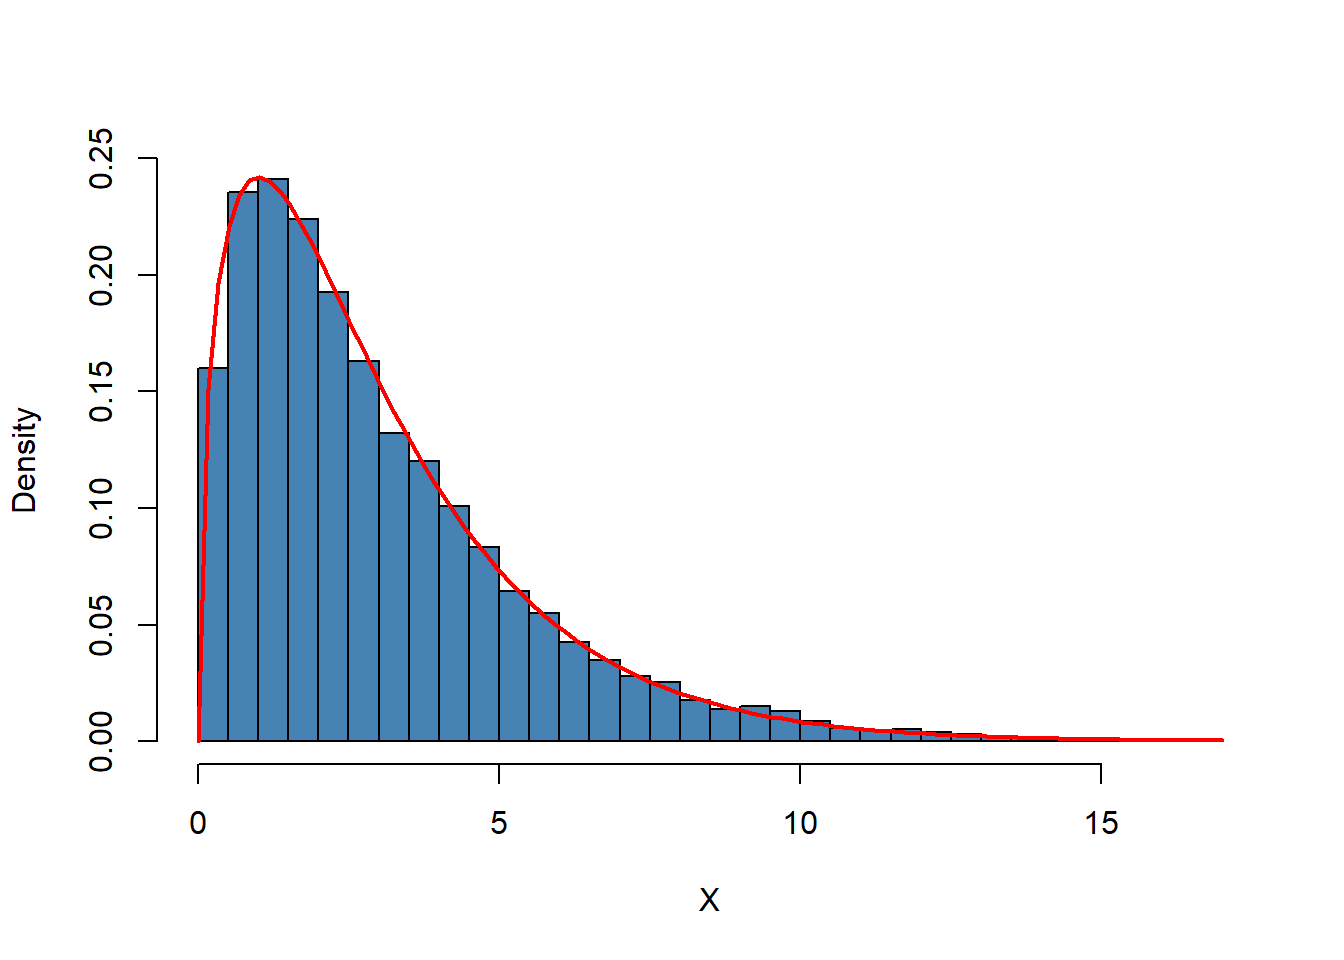
\includegraphics{URFITE_files/figure-latex/unnamed-chunk-37-1} \end{center}

We divide the plotting area up using \texttt{layout()}. The matrix
\texttt{m} specifies the locaion of the plots, see \texttt{?layout}.

We see that all relationships are negative. Here are the correlation
coefficients.

\begin{Shaded}
\begin{Highlighting}[]
\CommentTok{# estimate correlation between student characteristics and test scores}
\KeywordTok{cor}\NormalTok{(CASchools}\OperatorTok{$}\NormalTok{score, CASchools}\OperatorTok{$}\NormalTok{english)}
\end{Highlighting}
\end{Shaded}

\begin{verbatim}
## [1] -0.6441238
\end{verbatim}

\begin{Shaded}
\begin{Highlighting}[]
\KeywordTok{cor}\NormalTok{(CASchools}\OperatorTok{$}\NormalTok{score, CASchools}\OperatorTok{$}\NormalTok{lunch)}
\end{Highlighting}
\end{Shaded}

\begin{verbatim}
## [1] -0.868772
\end{verbatim}

\begin{Shaded}
\begin{Highlighting}[]
\KeywordTok{cor}\NormalTok{(CASchools}\OperatorTok{$}\NormalTok{score, CASchools}\OperatorTok{$}\NormalTok{calworks)}
\end{Highlighting}
\end{Shaded}

\begin{verbatim}
## [1] -0.6268533
\end{verbatim}

We shall consider five different model equations:

\begin{align*}
  (I) \quad TestScore=& \, \beta_0 + \beta_1 \times size + u, \\
  (II) \quad TestScore=& \, \beta_0 + \beta_1 \times size + \beta_2 \times english + u, \\
  (III) \quad TestScore=& \, \beta_0 + \beta_1 \times size + \beta_2 \times english + \beta_3 \times lunch + u, \\
  (IV) \quad TestScore=& \, \beta_0 + \beta_1 \times size + \beta_2 \times english + \beta_4 \times calworks + u, \\
  (V) \quad TestScore=& \, \beta_0 + \beta_1 \times size + \beta_2 \times english + \beta_3 \times lunch + \beta_4 \times calworks + u
\end{align*}

The best way to communicate regression results is in a table. The
\texttt{stargazer} package is very convenient for this purpose. It
provides a function that generates professionally looking HTML and LaTeX
tables that satisfy scientific standards. One simply has to provide one
or multiple object(s) of class \texttt{lm}. The rest is done by the
function \texttt{stargazer()}.

\begin{Shaded}
\begin{Highlighting}[]
\CommentTok{# load the stargazer library}
\KeywordTok{library}\NormalTok{(stargazer)}

\CommentTok{# estimate different model specifications}
\NormalTok{spec1 <-}\StringTok{ }\KeywordTok{lm}\NormalTok{(score }\OperatorTok{~}\StringTok{ }\NormalTok{size, }\DataTypeTok{data =}\NormalTok{ CASchools)}
\NormalTok{spec2 <-}\StringTok{ }\KeywordTok{lm}\NormalTok{(score }\OperatorTok{~}\StringTok{ }\NormalTok{size }\OperatorTok{+}\StringTok{ }\NormalTok{english, }\DataTypeTok{data =}\NormalTok{ CASchools)}
\NormalTok{spec3 <-}\StringTok{ }\KeywordTok{lm}\NormalTok{(score }\OperatorTok{~}\StringTok{ }\NormalTok{size }\OperatorTok{+}\StringTok{ }\NormalTok{english }\OperatorTok{+}\StringTok{ }\NormalTok{lunch, }\DataTypeTok{data =}\NormalTok{ CASchools)}
\NormalTok{spec4 <-}\StringTok{ }\KeywordTok{lm}\NormalTok{(score }\OperatorTok{~}\StringTok{ }\NormalTok{size }\OperatorTok{+}\StringTok{ }\NormalTok{english }\OperatorTok{+}\StringTok{ }\NormalTok{calworks, }\DataTypeTok{data =}\NormalTok{ CASchools)}
\NormalTok{spec5 <-}\StringTok{ }\KeywordTok{lm}\NormalTok{(score }\OperatorTok{~}\StringTok{ }\NormalTok{size }\OperatorTok{+}\StringTok{ }\NormalTok{english }\OperatorTok{+}\StringTok{ }\NormalTok{lunch }\OperatorTok{+}\StringTok{ }\NormalTok{calworks, }\DataTypeTok{data =}\NormalTok{ CASchools)}

\CommentTok{# gather robust standard errors in a list}
\NormalTok{rob_se <-}\StringTok{ }\KeywordTok{list}\NormalTok{(}
  \KeywordTok{sqrt}\NormalTok{(}\KeywordTok{diag}\NormalTok{(}\KeywordTok{vcovHC}\NormalTok{(spec1, }\DataTypeTok{type =} \StringTok{"HC1"}\NormalTok{))),}
  \KeywordTok{sqrt}\NormalTok{(}\KeywordTok{diag}\NormalTok{(}\KeywordTok{vcovHC}\NormalTok{(spec2, }\DataTypeTok{type =} \StringTok{"HC1"}\NormalTok{))),}
  \KeywordTok{sqrt}\NormalTok{(}\KeywordTok{diag}\NormalTok{(}\KeywordTok{vcovHC}\NormalTok{(spec3, }\DataTypeTok{type =} \StringTok{"HC1"}\NormalTok{))),}
  \KeywordTok{sqrt}\NormalTok{(}\KeywordTok{diag}\NormalTok{(}\KeywordTok{vcovHC}\NormalTok{(spec4, }\DataTypeTok{type =} \StringTok{"HC1"}\NormalTok{))),}
  \KeywordTok{sqrt}\NormalTok{(}\KeywordTok{diag}\NormalTok{(}\KeywordTok{vcovHC}\NormalTok{(spec5, }\DataTypeTok{type =} \StringTok{"HC1"}\NormalTok{)))}
\NormalTok{)}

\CommentTok{# generate a LaTeX table using stargazer}
\KeywordTok{stargazer}\NormalTok{(spec1, spec2, spec3, spec4, spec5,}
          \DataTypeTok{se =}\NormalTok{ rob_se,}
          \DataTypeTok{digits =} \DecValTok{3}\NormalTok{,}
          \DataTypeTok{header =}\NormalTok{ F,}
          \DataTypeTok{column.labels =} \KeywordTok{c}\NormalTok{(}\StringTok{"(I)"}\NormalTok{, }\StringTok{"(II)"}\NormalTok{, }\StringTok{"(III)"}\NormalTok{, }\StringTok{"(IV)"}\NormalTok{, }\StringTok{"(V)"}\NormalTok{)}
\NormalTok{          )}
\end{Highlighting}
\end{Shaded}

\begin{sidewaystable}[!htbp] \centering 
  \caption{\label{tab:rotsostracv} Regressions of Test Scores on the Student-Teacher Ratio and Control Variables} 
  \label{} 
\begin{tabular}{@{\extracolsep{-10pt}}lccccc} 
\\[-1.8ex]\hline 
\hline \\[-1.8ex] 
 & \multicolumn{5}{c}{Dependent Variable: Test Score} \\ 
\cline{2-6} 
\\[-1.8ex] & \multicolumn{5}{c}{score} \\ 
 & (I) & (II) & (III) & (IV) & (V) \\ 
\\[-1.8ex] & spec1 & spec2 & spec3 & spec4 & spec5\\ 
\hline \\[-1.8ex] 
 size & $-$2.280$^{***}$ & $-$1.101$^{**}$ & $-$0.998$^{***}$ & $-$1.308$^{***}$ & $-$1.014$^{***}$ \\ 
  & (0.519) & (0.433) & (0.270) & (0.339) & (0.269) \\ 
  & & & & & \\ 
 english &  & $-$0.650$^{***}$ & $-$0.122$^{***}$ & $-$0.488$^{***}$ & $-$0.130$^{***}$ \\ 
  &  & (0.031) & (0.033) & (0.030) & (0.036) \\ 
  & & & & & \\ 
 lunch &  &  & $-$0.547$^{***}$ &  & $-$0.529$^{***}$ \\ 
  &  &  & (0.024) &  & (0.038) \\ 
  & & & & & \\ 
 calworks &  &  &  & $-$0.790$^{***}$ & $-$0.048 \\ 
  &  &  &  & (0.068) & (0.059) \\ 
  & & & & & \\ 
 Constant & 698.933$^{***}$ & 686.032$^{***}$ & 700.150$^{***}$ & 697.999$^{***}$ & 700.392$^{***}$ \\ 
  & (10.364) & (8.728) & (5.568) & (6.920) & (5.537) \\ 
  & & & & & \\ 
\hline \\[-1.8ex] 
Observations & 420 & 420 & 420 & 420 & 420 \\ 
R$^{2}$ & 0.051 & 0.426 & 0.775 & 0.629 & 0.775 \\ 
Adjusted R$^{2}$ & 0.049 & 0.424 & 0.773 & 0.626 & 0.773 \\ 
Residual Std. Error & 18.581 (df = 418) & 14.464 (df = 417) & 9.080 (df = 416) & 11.654 (df = 416) & 9.084 (df = 415) \\ 
F Statistic & 22.575$^{***}$ (df = 1; 418) & 155.014$^{***}$ (df = 2; 417) & 476.306$^{***}$ (df = 3; 416) & 234.638$^{***}$ (df = 3; 416) & 357.054$^{***}$ (df = 4; 415) \\ 
\hline 
\hline \\[-1.8ex] 
\textit{Note:}  & \multicolumn{5}{r}{$^{*}$p$<$0.1; $^{**}$p$<$0.05; $^{***}$p$<$0.01} \\ 
\end{tabular} 
\end{sidewaystable}

Table \ref{tab:rotsostracv} states that \(scores\) is the dependent
variable and that we consider five models. We see that the columns of
Table \ref{tab:rotsostracv} contain most of the information provided by
\texttt{coeftest()} and \texttt{summary()} for the regression models
under consideration: the coefficients estimates equipped with
significance codes (the asterisks) and standard errors in parentheses
below. Although there are no \(t\)-statistics, it is straightforward for
the reader to compute them simply by dividing a coefficient estimate by
the corresponding standard error. The bottom of the table reports
summary statistics for each model and a legend. For an in-depth
discussion of the tabular presentation of regression results, see
Chapter 7.6 of the book.

What can we conclude from the model comparison?

\begin{enumerate}
\def\labelenumi{\arabic{enumi}.}
\item
  We see that adding control variables roughly halves the coefficient on
  \texttt{size}. Also, the estimate is not very sensitive to the set of
  control variables used. The conclusion is that decreasing the
  student-teacher ratio ceteris paribus by one unit leads to an
  estimated average increase in test scores of about \(1\) point.
\item
  Adding student characteristics as controls boosts \(R^2\) and
  \(\overline{R^2}\) from \(0.049\) (\texttt{spec1}) up to \(0.773\)
  (\texttt{spec3} and \texttt{spec5}), so we can consider these
  variables as suitable predictors for test scores. Moreover, the
  estimated coefficients on all control variables are consistent with
  the impressions gained from Figure 7.2 of the book.
\item
  We see that the control variables are not statistically significant in
  all models. For example in \texttt{spec5} we see that the coefficient
  on \(calworks\) is not significantly different from zero at the level
  of \(5\%\) since \(\lvert-0.048/0.059\rvert=0.81 < 1.64\). We also
  observe that the effect on the estimate (and its standard error) of
  the coefficient on \(size\) of adding \(calworks\) to the base
  specification \texttt{spec3} is negligible. We can therefore consider
  \texttt{calworks} as a redundant control variable in this model.
\end{enumerate}

\section{Exercises}\label{exercises}

\begin{center}\textit{This interactive part of URFITE is only available in the HTML version.}\end{center}

\bibliography{book.bib,packages.bib}


\end{document}
